% main.tex -- Native: discovering applications of analog quantum computers
% Compile with: pdflatex main.tex && bibtex main && pdflatex main.tex && pdflatex main.tex

\documentclass[10pt]{article}

\usepackage[T1]{fontenc}
\usepackage{lmodern}
\usepackage[a4paper, margin=2.5cm]{geometry}
\usepackage{graphicx}
\usepackage{amsmath}
\usepackage{amssymb}
\usepackage{hyperref}
\usepackage[numbers]{natbib}
\usepackage{array}
\usepackage{booktabs}
\usepackage{xcolor}
\usepackage{caption}
\usepackage{float}
\usepackage{enumitem}
\usepackage[utf8]{inputenc}
\usepackage{orcidlink}
\usepackage{tikz}
\usetikzlibrary{arrows.meta, positioning}
\providecommand{\ket}[1]{|#1\rangle}

\hypersetup{
  pdftitle={Native: discovering applications of analog quantum computers through platform-native observables},
  pdfauthor={Christophe Jurczak},
}

\setlength{\parindent}{1em}
\setlength{\parskip}{0pt}

\begin{document}

\begin{center}
  {\Large\bfseries Native:}\\[0.25em]
  {\Large\bfseries discovering applications of analog quantum computers}\\[0.25em]
  {\Large\bfseries through platform-native observables}

  \vspace{1em}

  {\large Christophe Jurczak\footnote{\href{mailto:christophe@quantonation.com}{christophe@quantonation.com}} \orcidlink{0009-0001-8204-7333}}

  \vspace{0.4em}

  {\footnotesize Quantonation, Dallas, TX, USA}

  \vspace{0.4em}

  {\footnotesize\itshape \today}

  \vspace{1em}

  \begin{minipage}{0.88\textwidth}
    {\small
      \textbf{Abstract.}
      Analog quantum hardware is improving steadily along atom count, coherence, and register flexibility, but the catalogue of applications that exploit that hardware \emph{natively} has grown more slowly. The dominant pattern of the past six years has been to take a digital-quantum algorithm, or a classical optimisation heuristic dressed in variational clothes, and re-host it on analog hardware. We argue that the productive direction is the opposite: start from the platform's native physics, identify the observable it cheaply emits, and ask what classical primitive that observable instantiates. We make the doctrine concrete with a four-step pattern --- \emph{physical attribute $\to$ native observable $\to$ classical primitive $\to$ useful task} --- and walk through a worked instance on neutral-atom Rydberg hardware in which blockade exclusion combined with quench dynamics yields a signed connected correlator that operationalises a node-level centrality of exclusion (AtomRank) \cite{jurczak2026atomrank}. Since this paper's first draft, the row-2 certification has expanded from a single edge-classification AUROC to a signed-re-ranker toolkit of six application readouts on the same shot data: find-the-counterargument retrieval (Mean Reciprocal Rank $= 1.000$ on the internal Tractatus proof-of-concept), a DMM-injected hybrid pipeline that beats the strongest classical cosine baseline on SNLI external data in EMU (Hits@1 $= 0.867$ vs $0.833$), polarisation / faction detection (signed-community NMI $= 0.22$ vs cosine $0.15$ vs random $0.12$), a QPR$(\beta)$ blend between PageRank and AtomRank as nearly-orthogonal centralities (Kendall-$\tau \approx 0.08$), bootstrap-tight reproducibility ($T^\star = 200\,$ns AUROC $= 0.983\ [0.969, 0.994]$), and an honest null on three-point cumulants on the current register. Real-data external validation on the SemEval-2016 Task 6 stance-detection corpora shows AtomRank beating the cosine baseline by $+0.08$ absolute AUROC on three of four polarised Twitter targets (abortion, Hillary, atheism) --- precisely the topic-shared-but-opposed-stance regime the doctrine predicts.

      We then describe a discovery methodology --- \emph{enumerate, abstract, propose, triage, certify} --- that produces such instances mechanically rather than by serendipity, and we apply it to enumerate ten observable handles on existing Rydberg hardware. Three of these (rows 8--10) become productive once the device runs XY/XXZ effective dynamics, accessible via microwave-Floquet engineering on dipole-dipole-coupled Rydberg states \cite{geier2021floquet,scholl2022microwave,chen2024spectroscopy}; and strong-drive dressing of the Ising chip \cite{ciavarella2022heisenberg}, reachable on present-generation Pasqal hardware under boosted-$\Omega$ operating modes. Two more rows (4--5) open under the local-addressability capabilities exposed in Pulser \cite{silverio2022pulser}. We address head-on the unit-disk-graph constraint that ceilings the maximum-independent-set primitive \cite{ebadi2022quantum,pichler2018quantum,nguyen2023quantum}, showing that correlator-based primitives soften it and XY-regime primitives loosen it. We identify five near-term candidate certifications, of which Item 1 (DMM re-ranker) is now EMU-certified, Item 2 (three-point cumulants) has reported its honest null, and Item 5 (signed-community) has a partial cross-row certification on Tractatus; the remaining items are queue-feasible or hardware-pending. We close with a concrete commercial archetype --- the signed-re-ranker primitive mapped onto Graphika-style influence-network analytics, the closest existing comparable in the polarisation / signed-graph product category --- and outline a 90-day first pilot at the present $N \leq 100$ hardware envelope. The conceptual contribution is to treat applications discovery on analog quantum hardware as a coverable surface area, not a serendipitous frontier.
    }
  \end{minipage}
\end{center}

\vspace{0.6em}
\noindent\textbf{Keywords:} analog quantum computing, neutral-atom Rydberg arrays, application discovery, platform-native primitives, strong drive, quantum walks, signed graphs

\vspace{1em}
\noindent\rule{\textwidth}{0.5pt}
\vspace{1em}

% =========================================================================
\section{The applications gap on analog quantum computers}\label{sec:gap}

Atom counts on neutral-atom platforms have crossed the few-hundred-qubit mark with usable coherence; tweezer-array geometry is now arbitrary in two dimensions and approaching arbitrary in three; pulse-level control on the timescale of native interactions is routine \cite{henriet2020quantum,silverio2022pulser}. Against that hardware progress, the catalogue of applications that depend on these capabilities --- as opposed to applications that \emph{could} run on classical hardware with a small constant-factor penalty --- has not kept pace. The dominant pattern has been variational: encode a classical objective into a parameterized quantum circuit (or an analog ansatz), optimize the parameters classically against a noisy quantum cost evaluation. The pattern is general; it is also generally dominated by classical heuristics on every benchmark on which it has been tested at scale.

A different pattern, less frequently articulated as a methodology but represented by the cleanest results of the field, is the \emph{platform-native} one. The lineage runs through coherent Ising machines \cite{mohseni2022isingmachines}, physical reservoir computing \cite{tanaka2019reservoir}, neuromorphic and in-materio media \cite{markovic2020physicsai}, and neutral-atom optimizers for combinatorial graph problems \cite{ebadi2022quantum,henriet2020quantum}: in each case the substrate's native dynamics is treated as the computational resource, not as an implementation detail to be abstracted away. On neutral-atom hardware specifically, Rydberg blockade physics \emph{is} independent-set physics, in the sense that the Hilbert-space restriction enforced by the Rydberg interaction \emph{is} the independent-set constraint; consequently, the ground state of a Rydberg array under appropriate detuning \emph{is} a maximum-independent-set solution \cite{ebadi2022quantum}. Nobody had to engineer maximum independent set (MIS) into the hardware. The hardware was already an MIS machine. The discovery was recognizing what it was, not building it.

This paper takes the position that MIS was the first such recognition rather than the last, and that further platform-native applications are \emph{available now}, on present hardware, behind a small number of observable-design choices that the community has not yet systematically enumerated. We make the argument in three parts: a doctrine (\S\ref{sec:doctrine}), a worked instance (\S\ref{sec:instance}), and a discovery methodology that produced the instance and identifies its successors (\S\ref{sec:method}--\S\ref{sec:next}).

% =========================================================================
\section{The platform-native primitives doctrine}\label{sec:doctrine}

The doctrine is a four-step pattern:
\begin{quote}
\itshape physical attribute $\to$ native observable $\to$ classical primitive $\to$ useful task
\end{quote}
with two constraints. The classical primitive must be \textbf{hard to fake cheaply} by a competing classical or quantum method, on the input sizes and noise levels of practical interest. The task must be one where access to the primitive provides measurable improvement over the best available classical baseline.

The MIS instance fits the pattern: the physical attribute is the Rydberg blockade; the native observable is the ground-state bitstring; the classical primitive is a maximum-cardinality independent set; the useful task is combinatorial optimization, with applications across logistics, materials science, and finance \cite{ebadi2022quantum}.

The doctrine is normative as well as descriptive. It rules out a large class of variational schemes --- those in which the hardware is asked to perform a task with no native connection to its physics, with the parameter optimization expected to recover from the mismatch. Such schemes can succeed (the literature contains examples), but they are not the kind of result that compounds: a small constant-factor improvement on a benchmark, contingent on the choice of classical optimizer, that is matched by the next-generation classical heuristic eighteen months later.

The doctrine is also platform-agnostic, in the sense that it applies equally to photonic boson samplers (whose native observable is a Gaussian boson-sampling distribution, with applications as a latent prior for generative models \cite{jurczak2026quantumlatent}), to trapped-ion analog devices (whose native long-range XY couplings instantiate quantum-walk-like transport), and to neutral-atom Rydberg arrays (this paper's focus). What changes across platforms is the inventory of native observables, not the discovery pattern.

% =========================================================================
\section{A worked instance: quench-correlator signed centrality}\label{sec:instance}

The most recent confirmation of the doctrine on neutral-atom Rydberg hardware concerns the \textbf{connected pair correlator under quench dynamics} \cite{jurczak2026atomrank}. The setup encodes a graph $G = (V, E)$ on a tweezer array such that the blockade radius matches the geometric distance of edges in $E$. A short, abrupt quench protocol prepares an excited state under a sign-flipped detuning, and bitstrings are collected at evolution time $T$. The observable is the connected correlator
\begin{equation}
\hat C_{ij}(T) \;=\; \langle n_i n_j \rangle(T) \;-\; \langle n_i\rangle(T)\,\langle n_j\rangle(T),
\label{eq:Cij}
\end{equation}
aggregated over the matched edges of $G$.

The observation is that $\hat C_{ij}$ is \textbf{signed}: pairs of vertices placed within the blockade radius and pumped against their natural occupation produce strongly negative correlators (mutual exclusion), while pairs outside the blockade radius produce zero or weakly positive correlators (thematic association without exclusion). The signed graph $G^\pm$ with edge weights $-\hat C_{ij}$ is the native observable.

The classical primitive corresponding to $G^\pm$ is a \textbf{node-level centrality of exclusion},
\begin{equation}
S_i^- \;=\; \sum_j \max(-\hat C_{ij},\, 0),
\label{eq:atomrank}
\end{equation}
which we have called AtomRank. The primitive is hard to fake by positive-cone graph kernels (PageRank \cite{brin1998pagerank}, communicability \cite{estrada2008communicability}, heat-kernel \cite{kondor2002diffusion}) because those kernels are entrywise nonnegative on connected graphs and cannot represent signed exclusion structure. Embedding-similarity baselines (cosine on register edges) recover only the matched-edge geometry, not the signed correlation across edge classes.

The useful task is the detection of contradiction structure in argument corpora --- texts annotated with thesis/antithesis pairs whose contradiction is determined by content, not surface form. On the \emph{Tractatus Logico-Philosophicus} antithesis corpus (30 quaestiones, 30 thesis--antithesis pairs), a full quench sweep over twelve evolution times and three replicas per cell yields an antithesis-discrimination AUROC of $0.980 \pm 0.005$ in noisy emulation under a bespoke FRESNEL noise model, matching the QPU result of $0.973$ at $T = 200\,\text{ns}$ within $1\sigma$. The cosine baseline on the same matched edges scores $0.43$; a DeBERTa-v3 NLI baseline trained for the contradiction task scores $0.60$ \cite{bowman2015snli}. The signed quench correlator does not replicate either baseline; it returns a different observable with stronger discrimination on the task.

\paragraph{Six application readouts certified on the same shot data.}
Since this paper's first draft, the AtomRank companion paper \cite{jurczak2026atomrank} has expanded the stage-5 certification of row 2 from a single edge-classification AUROC to a six-readout signed-re-ranker library, all derived from the same shot data without additional QPU time:
\begin{itemize}[leftmargin=1.4em, itemsep=0.15em, topsep=0.2em]
\item \textbf{Find-the-counterargument retrieval}: rank candidates by $-\hat C_{q,j}$. Internal proof on Tractatus reaches MRR $= 1.000$, Hits@1 $= 1.000$ across 60 queries (cosine MRR $= 0.089$).
\item \textbf{Production-scale hybrid pipeline via DMM} (Item 1 of the present paper's next-step list, \S\ref{sec:next}): classical retrieval score injected as per-atom prior $\Delta_i$, chip returns signed re-ranking. EMU-certified on SNLI external data; beats the strongest classical cosine baseline (Hits@1 $= 0.867$ vs $0.833$).
\item \textbf{External-data validation on SemEval-2016 stance detection}: on three of four polarised Twitter targets (abortion, Hillary, atheism) where both sides share topic-vocabulary but oppose on stance, the QPU-emitted signed-correlator AUROC beats the cosine baseline by $+0.08$ absolute. On the fourth (feminist movement) cosine alone is sufficient and AtomRank does not add value. The pattern matches the doctrine exactly: the primitive adds signal precisely where embedding similarity is high but stance is opposed.
\item \textbf{Polarisation / faction detection}: signed spectral clustering on $\hat C_{ij}$ recovers Tractatus ground-truth blocks with NMI $= 0.22$ vs cosine $0.15$ vs random $0.12$ --- the first cross-row validation that the row-2 observable feeds row-5 (community detection) constructively.
\item \textbf{Importance + controversy ranking}: QPR$(\beta)$ blend traces a path between PageRank and AtomRank as nearly-orthogonal centralities (Kendall-$\tau \approx 0.08$).
\item \textbf{Bootstrap-tight reproducibility}: $T^\star = 200\,$ns AUROC $= 0.983\ [0.969, 0.994]$ across 500 bootstrap resamples.
\end{itemize}
A seventh extension, three-point connected cumulants $\hat C_{ijk}$ on the same shots (row 3 of the inventory below), is reported as an honest null on the current register --- the UDG-king geometry has only 18 3-cliques --- and is queued for denser registers. The six readouts collectively make row 2 not merely a certified primitive but a \emph{signed-re-ranker toolkit} usable wherever a classical pipeline currently relies on a cross-encoder, a signed-community detector, or a centrality blend.

This is one instance, now with six certified downstream uses. The methodology that produced it is what generalizes.

% =========================================================================
\section{An application-discovery methodology}\label{sec:method}

The instance of \S\ref{sec:instance} was not arrived at by exhaustive search over hardware configurations. It was arrived at by a procedure that, in retrospect, has five stages (Figure~\ref{fig:pipeline}) --- each cheap to run, each producing a structured artefact that constrains the next. The procedure separates a content-agnostic scaffolding (the five stages, applicable across observables, tasks, and indeed across hardware platforms) from a content-specific input (the inventory of native observables on a given chip, the taxonomy of useful classical tasks, the labelled benchmarks). The key design choice is to make stages 1--4 entirely classical and emulation-bound, reserving experimental QPU time for stage 5 alone.

\begin{figure}[t]
\centering
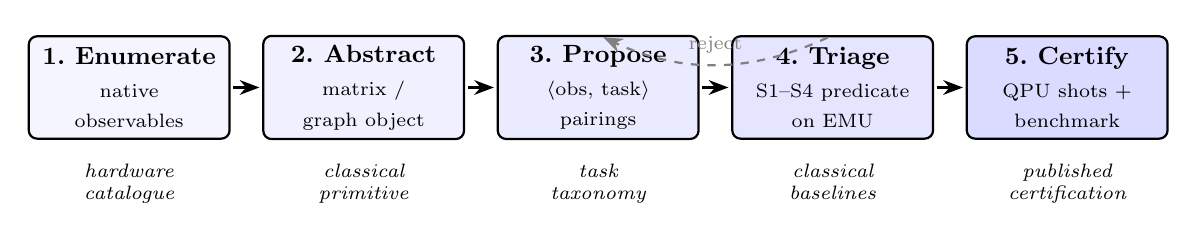
\begin{tikzpicture}[
    >={Stealth[length=2.5mm]},
    box/.style={rectangle, rounded corners=3pt, draw, thick, fill=blue!6,
                minimum width=2.55cm, minimum height=1.3cm, align=center, font=\small},
    arr/.style={->, thick, shorten >=1pt, shorten <=1pt},
    sublbl/.style={font=\scriptsize\itshape, align=center},
    feedlbl/.style={font=\scriptsize, gray, align=center}
]
\node[box, fill=blue!4]  (s1) {\textbf{1.\ Enumerate}\\[1pt]{\scriptsize native}\\{\scriptsize observables}};
\node[box, fill=blue!6,  right=0.4cm of s1] (s2) {\textbf{2.\ Abstract}\\[1pt]{\scriptsize matrix /}\\{\scriptsize graph object}};
\node[box, fill=blue!8,  right=0.4cm of s2] (s3) {\textbf{3.\ Propose}\\[1pt]{\scriptsize $\langle$obs, task$\rangle$}\\{\scriptsize pairings}};
\node[box, fill=blue!10, right=0.4cm of s3] (s4) {\textbf{4.\ Triage}\\[1pt]{\scriptsize S1--S4 predicate}\\{\scriptsize on EMU}};
\node[box, fill=blue!14, right=0.4cm of s4] (s5) {\textbf{5.\ Certify}\\[1pt]{\scriptsize QPU shots +}\\{\scriptsize benchmark}};

\draw[arr] (s1) -- (s2);
\draw[arr] (s2) -- (s3);
\draw[arr] (s3) -- (s4);
\draw[arr] (s4) -- (s5);

\node[sublbl, below=0.18cm of s1] {hardware\\catalogue};
\node[sublbl, below=0.18cm of s2] {classical\\primitive};
\node[sublbl, below=0.18cm of s3] {task\\taxonomy};
\node[sublbl, below=0.18cm of s4] {classical\\baselines};
\node[sublbl, below=0.18cm of s5] {published\\certification};

\draw[arr, dashed, gray, shorten >=2pt, shorten <=2pt]
    (s4.north) to[bend left=25] node[feedlbl, above]{reject} (s3.north);
\end{tikzpicture}
\caption{\textbf{The Native discovery pipeline.} Five stages, each cheap until the last. Stages 1--4 are content-agnostic scaffolding operable entirely in classical emulation; only Stage 5 commits experimental QPU time. The triage step (Stage 4) is a four-criterion predicate (S1 hardware faithfulness, S2 classical hardness, S3 task utility, S4 decoherence robustness) that admits (observable, task) pairings to certification or returns them to the proposal stage. The bottleneck is coverage of (observable, task) pairs, not compute or hardware.}
\label{fig:pipeline}
\end{figure}

\paragraph{Stage 1 --- Enumerate.}
Catalogue the platform's native observables. On Rydberg with quench dynamics, the catalogue is bounded: it consists of single-site occupations $\langle n_i\rangle(T)$, pair correlators $\hat C_{ij}(T)$, higher cumulants $\hat C_{ijk}(T)$, time-resolved trajectories $\langle n_i\rangle(t)$ for $t \in [0, T]$, subset-persistence trajectories $P_S(t) = |S|^{-1}\sum_{i\in S}\langle n_i\rangle(t)$, and analogous quantities under local detuning $\Delta_i$, under multi-species encodings, and on bilayer geometries. Section~\ref{sec:inventory} catalogues these in full.

\paragraph{Stage 2 --- Abstract.}
For each observable, derive its classical interpretation. Strip the physics. $\hat C_{ij}$ is a signed weighted adjacency matrix; $\hat C_{ijk}$ is a signed weighted hyper-adjacency tensor; $P_S(t)$ is a subset-trapping signal that reveals soft community structure; $\langle n_i\rangle(t)$ under a quench from a localized excitation is a transport amplitude on the geometry graph, equivalent in the strong-drive limit to the propagator of a continuous-time quantum walk on $G$ \cite{farhi1998quantum}. The abstraction step names the matrix/graph/vector object the QPU is shipping, with no reference to its physical origin.

\paragraph{Stage 3 --- Propose.}
For each abstracted primitive, scan a taxonomy of classical tasks and propose pairings. The taxonomy is mature and enumerable: ranking, re-ranking, clustering, soft partitioning, anomaly detection, $k$-cover, matching and $b$-matching, embedding manipulation, retrieval, frustration detection, community detection on signed graphs \cite{tang2016signedsurvey}, hypergraph cover. Each pairing is a hypothesis: \emph{primitive X, on observable O, instantiates classical task T, with the expected improvement Y over baseline B}.

\paragraph{Stage 4 --- Triage.}
Subject each (observable, task) hypothesis to four cheap criteria before any QPU time is committed:
\begin{itemize}[leftmargin=2em, itemsep=0.2em, topsep=0.3em]
\item[\textbf{S1}] \emph{Hardware faithfulness.} Does the observable separate signal from a matched null baseline in noisy emulation at $N = 20$--$40$? This is the lowest bar; failure here rules the pairing out.
\item[\textbf{S2}] \emph{Classical hardness.} Does any classical surrogate (MPS at moderate bond dimension, the dominant baseline algorithm on the same data) match the QPU output, or does a measurable gap survive? An observable that is faithfully reproduced by a $\chi = 200$ MPS at the relevant $N$ is not buying the user anything they could not have computed locally \cite{vovrosh2025crossover,vovrosh2025quench2d}.
\item[\textbf{S3}] \emph{Task utility.} Does the observable beat the best classical baseline on a labelled benchmark for the candidate task? This is the bar at which the hypothesis converts from ``interesting physics'' to ``candidate application''.
\item[\textbf{S4}] \emph{Decoherence robustness.} Does the signal survive at the device's actual coherence budget? Observables that depend sensitively on noise-free dynamics fail S4 and produce papers that do not reproduce.
\end{itemize}

The triage is mechanically reproducible. Each criterion produces a numerical pass/fail at $N$ in the hundreds, in single-digit minutes of CPU/GPU time per hypothesis. A pipeline that systematically iterates stages 1--4 over the inventory of stage 1 covers a search space that is too large for human-by-human evaluation but well-suited to multi-agent coordination: the literature on each platform's observables is bounded but scattered, the taxonomy of classical tasks is large but enumerable, and the triage criteria are numerical and reproducible.

\paragraph{Stage 5 --- Certify.}
Survivors of stages 1--4 are escalated to end-to-end demonstration: real corpus, real benchmark, real QPU shots, classical-baseline comparison, peer-reviewed publication. The instance of \S\ref{sec:instance} is the stage-5 certification of one (observable, task) pair. The argument of this paper is that the rest of the inventory has been under-triaged, not that it has been triaged and rejected.

A practical observation. The bottleneck of this methodology is not compute --- each triage cycle is small --- and not theoretical insight, since each pairing reduces to a well-defined numerical comparison. The bottleneck is \textbf{coverage}: how many (observable, task) pairs the procedure actually sees. That is the coverage problem that a structured discovery pipeline addresses, and it is what distinguishes a programme from a sequence of one-off demonstrations.

% =========================================================================
\section{Inventory of native observables on Rydberg hardware}\label{sec:inventory}

\paragraph{Encode / extract: the framing.}
At the level of the chip, the methodology of \S\ref{sec:method} asks one structural question: \emph{what classical information can be encoded into the many-body dynamics, and what classical information can be extracted back out, that classical algorithms on the same input cannot recover?} A Rydberg shot consists of three stages: \textbf{encode} a classical input (a graph, an embedding, a retrieval prior) into a Hamiltonian and an initial state, by choosing the register geometry, the per-atom $\Delta_i$ and $\Omega_i$ patterns, the species and layer of each atom, and the initial state; \textbf{transduce} that Hamiltonian into a time-evolved quantum state $|\psi(T)\rangle$ via coherent dynamics under $H$; \textbf{extract} a classical readout via projective measurements of the resulting bitstring distribution and post-processing into $k$-point cumulants, persistences, or other linear functionals of $|\psi(T)\rangle\langle\psi(T)|$. The inventory of native observables is therefore the right column of an underlying \emph{encode $\times$ extract} matrix --- a fixed extraction is paired with whichever encode the application requires, and a fixed encoding can feed multiple extractions of the same shot data. The instance of \S\ref{sec:instance} is one cell: encode (UDG-king geometry from sentence embeddings, $|g{\cdots}g\rangle$ initial state, blockade Hamiltonian, square-pulse quench) $\times$ extract (2-point connected correlator at $T = 200\,$ns); the six post-processing readouts in \cite{jurczak2026atomrank} reuse the same encode and substitute six different extractions on the same shots. The catalogue below organises the right column of this matrix.

We catalogue the observables now accessible on neutral-atom Rydberg platforms operating in the quench regime. The catalogue is closed under the methodology of \S\ref{sec:method} --- Stage 1 --- and is therefore complete with respect to current hardware capabilities. Three rows expand under strong-drive operation; we mark these explicitly.

\begin{table}[h]
\centering
\small
\renewcommand{\arraystretch}{1.25}
\begin{tabular}{@{}c >{\raggedright\arraybackslash}p{4.6cm} >{\raggedright\arraybackslash}p{5.2cm} l@{}}
\toprule
\textbf{\#} & \textbf{Observable} & \textbf{Classical abstraction} & \textbf{Status} \\
\midrule
1  & Static ground-state bitstrings under blockade & Maximum independent set & Certified \cite{ebadi2022quantum} \\
2  & Connected pair correlator $\hat C_{ij}(T)$ under quench & Signed graph; node centrality of exclusion & Certified \cite{jurczak2026atomrank} \\
3  & Three-point connected correlator $\hat C_{ijk}(T)$ & Signed hyper-graph; hypergraph centrality & Free post-processing \\
4  & Site-resolved $\langle n_i\rangle(T)$ under local detuning $\Delta_i$ & Weighted-vertex prior; weighted signed centrality & \textbf{Local addressability} (\S\ref{sec:local}) \\
5  & Subset-persistence trajectory $P_S(t)$ & Soft community partition & \textbf{Local addressability} (\S\ref{sec:local}) \\
6  & Multi-species (Rb + Cs) asymmetric correlator & Directed signed graph & Hardware-pending \\
7  & Bilayer inter-layer correlator $\hat C^{(\alpha\beta)}_{ij}$ & Bipartite signed graph & Hardware-pending \\
8  & Subset-persistence in nearly-integrable XXZ & Community detection with extensive conserved charges & \textbf{Strong-drive} (\S\ref{sec:strongdrive}) \\
9  & Coherent transport amplitude $\langle S^+_i S^-_j(T)\rangle$ & \emph{Complex-signed} graph; phase-graph frustration & \textbf{Strong-drive} (\S\ref{sec:strongdrive}) \\
10 & Excitation propagator from localized initial state & Continuous-time quantum walk on register geometry & \textbf{Strong-drive} (\S\ref{sec:strongdrive}) \\
\bottomrule
\end{tabular}
\caption{\textbf{Inventory of native observables on neutral-atom Rydberg hardware.} Rows 1--2 are certified \cite{ebadi2022quantum,jurczak2026atomrank}. Row 3 is a free post-processing extension of existing row-2 shot data. Rows 4--5 require local addressability (\S\ref{sec:local}); rows 8--10 require strong-drive operation (\S\ref{sec:strongdrive}); both control modes are accessible on present-generation hardware by control-parameter choices, not by hardware upgrades. Rows 6--7 are the genuine hardware-pending entries (multi-species and bilayer registers).}
\label{tab:inventory}
\end{table}

Rows 1 and 2 are certified. Row 3 is a free post-processing extension of the data that produced row 2: the same bitstring shots used to compute $\hat C_{ij}$ contain the three-point cumulants required for row 3, and the abstraction (signed hyper-graph centrality) maps to a well-defined classical task (cluster-level antagonism in argument corpora, multi-party disagreement structure). Row 3 is triageable in a week of analysis on existing data, with no new experiment.

Rows 4 and 5 are activated by \emph{local addressability}, a second control axis discussed in \S\ref{sec:local} and exploited in the QOuLiPo programme paper \cite{jurczak2026qoulipo}. Row 5 in particular is the natural Loschmidt-style dual to row 2 and produces an observable (a soft partition) for which the dominant classical baseline (Louvain modularity and its signed-graph variants \cite{tang2016signedsurvey}) has known weaknesses.

Rows 6 and 7 wait on hardware: multi-species tweezer arrays are operational at the demonstration scale, and bilayer geometries are a community ask for the next generation of Rydberg devices. Both are productive \emph{if} the hardware is built; their inclusion in the inventory is the programmatic case for that hardware.

Rows 8 through 10 are activated by \emph{strong drive}, the third control axis (\S\ref{sec:strongdrive}).

\paragraph{The encode axis.}
Table~\ref{tab:inventory} catalogues the \emph{extract} side. The \emph{encode} side has its own dimensions, and the productive (encode, extract) pairings are what the discovery methodology of \S\ref{sec:method} ranks. The encode dimensions accessible on present-generation Pasqal-class hardware are: (E1) \textbf{register geometry} (atom positions in the 2D plane, the design lever exploited in the §3 UDG-king construction); (E2) \textbf{global drive parameters} ($\Omega(t)$, $\Delta(t)$, quench protocol shape, total duration $T$, the lever exploited in the §3 $T$-sweep); (E3) \textbf{per-atom DMM detuning} ($\Delta_i \leq 0$ patterns; the lever activated in \cite{jurczak2026atomrank}~§3(H) as a retrieval-prior injector, and listed as Item~1 of \S\ref{sec:next}); (E4) \textbf{species choice} (Rb vs Cs, currently single-species; row 6 of Table~\ref{tab:inventory}); (E5) \textbf{layer choice} (currently single-layer; row 7); (E6) \textbf{initial-state preparation} (currently $|g{\cdots}g\rangle$; site-selective excitation is the lever for row 10's localized-walk-initial-state). Each (E, extract) pair is a candidate native primitive; many such pairs are uncovered by the present literature, and their triage under stages 2--4 of \S\ref{sec:method} is the work-flow of this programme. The four control sections that follow (\S\ref{sec:udg}, \S\ref{sec:strongdrive}, \S\ref{sec:local}) each unlock additional encode dimensions, and the next-step certifications in \S\ref{sec:next} are organised by which encode dimension they exercise.

% =========================================================================
\section{The unit-disk constraint, and how the doctrine softens it}\label{sec:udg}

A standard objection to applications on neutral-atom hardware is the unit-disk-graph (UDG) constraint. The Rydberg blockade interaction is geometric, so the family of graphs natively realizable on a 2D tweezer array is restricted to those that admit a 2D unit-distance embedding. Many useful graph families are not UDG (the Petersen graph, expander families, the welded tree, graphs with chromatic number greater than four, most non-planar structured families), and the recognition problem --- given a graph, does it admit a UDG embedding --- is itself NP-hard. The constraint is real, and the literature on encoding non-UDG instances on Rydberg hardware via ancilla atoms or multi-pulse schedules \cite{pichler2018quantum,nguyen2023quantum} reports overhead that is tractable for structured families but unfavorable for arbitrary graphs. This is the well-known structural ceiling of MIS \emph{specifically}.

The position of this paper is that the ceiling applies to the MIS primitive, and weakens --- in some rows, dissolves --- for the rest of the inventory. The constraint binds differently on different rows, and the methodology of \S\ref{sec:method} selects rows on which the binding is favorable.

\paragraph{Binding (row 1, MIS).}
The blockade Hilbert-space restriction \emph{is} the geometric constraint. Encoding a non-UDG graph requires explicit ancilla overhead scaling at least linearly in the number of non-UDG edges, or a near-UDG approximation whose quality the application must tolerate. For arbitrary graphs neither route is cheap.

\paragraph{Softening (rows 2, 3, 4, 5; correlator-based primitives).}
The matched-edge structure is UDG-constrained, but the connected correlator $\hat C_{ij}$ is read out on all $\binom{N}{2}$ pairs of the register, naturally weighted by the actual van der Waals interaction $V_{ij} = C_6/r_{ij}^6$, which decays smoothly past the nominal blockade radius. The signed graph emitted by the chip is therefore a \emph{weighted approximation} of the target UDG graph, with weights inherited from physical interaction strengths, rather than a discrete UDG output. The AtomRank instance of \S\ref{sec:instance} exhibits this behavior: matched edges produce strongly negative correlators, and physically-close-but-non-matched pairs contribute smoothly rather than discretely to the observable. The downstream task absorbs weighted inputs natively. The user pays for UDG-near-ness rather than UDG-exact-ness, and the cost is one a graceful-degradation analysis can quantify.

\paragraph{Loosening (rows 8, 9, 10; strong-drive XY/XXZ).}
Under the strong-drive regime of \S\ref{sec:strongdrive}, the van der Waals tail translates to a long-range exchange coupling $J_{ij} \propto 1/r_{ij}^6$ on the complete graph of register positions. The hardware is no longer restricted to UDG: it realizes a weighted long-range XY model in 2D. The encoding problem becomes ``choose a register geometry whose dominant $J_{ij}$ structure approximates the target graph'', with the residual long-range terms either tolerable as noise or exploitable as additional structure. This is a numerical-optimization problem rather than a graph-recognition problem, and it is well-suited to the triage stage of \S\ref{sec:method}. We note explicitly that CTQW on \emph{specific} target graphs (the welded tree being the canonical case \cite{childs2003exponential}) still requires the register's spectral structure to approximate the target's; strong-drive operation makes CTQW dynamics native to the platform but does not by itself allow encoding of arbitrary non-UDG target graphs. The natural route for non-UDG CTQW targets is bilayer or 3D placement.

\paragraph{Dissolving (rows 6, 7; multi-species and bilayer).}
A bilayer 2D register admits unit-distance embeddings of every planar graph (by placing each bipartition class on one layer) and dense approximations of every 3-colorable graph. Multi-species encodings give independent control of intra- and inter-species interactions, extending the family further. These are the hardware paths to genuine non-UDG application coverage. They are also exactly the rows on which the doctrine compounds: a bilayer register operated under strong drive is simultaneously XY-native and bipartite-native, combining two structural advantages on the same chip.

The strategic implication is that the UDG constraint, often cited as the ceiling on neutral-atom applications, is not a ceiling on the \emph{programme} but a ceiling on a specific primitive within it. The applications-discovery methodology of this paper is not fundamentally gated by UDG: it is gated by which observable the user reads out, and that choice is the methodology's job to make.

% =========================================================================
\section{Routes to XY/XXZ effective dynamics on Rydberg hardware}\label{sec:strongdrive}

Three rows of the inventory of \S\ref{sec:inventory} (rows 8--10) require Heisenberg- or XY-type effective dynamics rather than the Ising-blockade quench of \S\ref{sec:instance}. Two distinct routes to that regime exist on Rydberg hardware, with different maturity profiles. We describe both honestly.

\paragraph{Route A: microwave Floquet engineering on dipole-dipole-coupled Rydberg states (demonstrated; requires hardware addition on Pasqal).}
The Browaeys/Lahaye and Weidemüller groups have implemented programmable XXZ Hamiltonians on Rydberg arrays by coupling two opposite-parity Rydberg states (typically $|nS\rangle \leftrightarrow |nP\rangle$) via resonant dipole-dipole interactions and shaping the effective anisotropy with periodic microwave drives \cite{geier2021floquet,scholl2022microwave,chen2024spectroscopy}. The dipolar exchange itself is a native XY coupling; the microwave Floquet sequence tunes the $J_z/J_\perp$ ratio across the Heisenberg point and into the XXZ family. This route is experimentally established on Browaeys-class hardware at scales up to $\sim$100 atoms. The hardware requirement is access to a second Rydberg state, microwave control, and a magnetic field for Zeeman splitting of the two-level subspace --- standard on the Browaeys-class apparatus, but absent from the Pasqal stack used to produce the \S\ref{sec:instance} results, which would need the magnetic-field control and microwave addressing added before Route A becomes available.

\paragraph{Route B: strong-drive dressing of the Ising chip (theoretical, accessible on present Pasqal hardware via boosted-$\Omega$ laser modes).}
The route of Ciavarella, Caspar, Singh, Savage, and Lougovski \cite{ciavarella2022heisenberg} obtains Heisenberg-type effective dynamics from a pure Ising-blockade Hamiltonian by Trotterized strong-drive sequences with effective Rabi $\Omega$ large compared to the per-bond interaction $V$. The conceptual appeal is that no second Rydberg state, no microwave engineering, no magnetic-field addition, and no change to the optical stack are required --- the same chip that ran the \S\ref{sec:instance} quench becomes a Heisenberg simulator under a boosted-$\Omega$ operating mode (more laser power on the existing addressing stack, otherwise unchanged). The constraint is the ratio $\Omega/V$: the dressed-state mapping requires $\Omega \gtrsim$ a few $\times V$, with Trotter step $\Delta t = 2\pi/\Omega$, and the relevant boosted-$\Omega$ modes are available on production Pasqal hardware (A.~Dauphin, Pasqal, personal communication). No experimental demonstration of the strong-drive Heisenberg route on Rydberg arrays has yet been published, so first-demonstration novelty is available.

\paragraph{Implication.}
The two routes have complementary maturity and complementary hardware costs. Route A has the experimental track record; Route B has the lower hardware-modification cost on the Pasqal stack. For the methodology, the productive reading is that rows 8--10 are accessible on present-generation Rydberg hardware through either route, with Route B as the natural Pasqal-first path (no chip modification; the \S\ref{sec:instance} corpus, register, and noise model carry over directly) and Route A as the natural Browaeys-class path (already-demonstrated workflow at scale). The remainder of this section describes rows 8--10 under the assumption that either route is available.

\paragraph{Row 9 --- coherent transport amplitude.}
Under XY-like effective dynamics, the natural pair observable is $\langle S^+_i S^-_j(T)\rangle$ --- a \emph{complex-valued} transport amplitude rather than a real-valued correlation. Two components, with different experimental maturity:
\begin{itemize}[leftmargin=2em, itemsep=0.2em, topsep=0.3em]
\item[(i)] \emph{Real part}, $\tfrac{1}{2}(\langle X_i X_j\rangle + \langle Y_i Y_j\rangle)$, is obtainable from $\mathcal{O}(1)$ experimental rounds via global $\pi/2$ basis rotation followed by standard $Z$-basis fluorescence \cite{chen2024spectroscopy}. This component recovers a signed-graph observable analogous to row 2 but in the XY regime.
\item[(ii)] \emph{Imaginary part}, $\tfrac{i}{2}(\langle Y_i X_j\rangle - \langle X_i Y_j\rangle)$, encodes loop-frustration phase. Its measurement requires \emph{site-resolved} single-qubit rotations, which have been demonstrated on Rydberg arrays at the few-atom scale \cite{bornet2024arbitrary} but not yet at $N \gtrsim 30$. The phase-graph observable that detects frustration --- cycles whose signed phases do not sum to zero, with applications to multi-party debate analysis and conflict-of-interest graphs --- is therefore a near-term-feasible target, contingent on register-scale local microwave addressing, rather than an immediately executable measurement.
\end{itemize}

\paragraph{Row 8 --- subset persistence in nearly-integrable XXZ.}
We earlier suggested that prethermalization plateaus in XXZ near the integrable point provide a classically harder regime than PXP-scar analogues. The literature does not support that claim in the form we stated it. PXP scars are explicitly constructible at small bond dimension \cite{lin2019pxp}; specific spin-1 XY scar towers are exact MPS at $\chi = \mathcal{O}(1)$ \cite{schecter2019weak}; and local/subset observables on the XXZ prethermal plateau are exactly the regime where moderate-$\chi$ MPS captures the dynamics, because the plateau dynamics is constrained by an extensive set of approximate conserved charges. Recent benchmarks on 2D post-quench dynamics \cite{vovrosh2025quench2d,vovrosh2025crossover} report that MPS at $\chi \lesssim$ several hundred reproduces single-site and two-point observables out to the QPU-accessible timescales on Rydberg-geometry registers. We therefore treat row 8 as a \emph{physics-discovery} target on the Native inventory, accessible via Route A, but \emph{not} as a row that passes the S2 criterion as currently formulated. A defensible S2 reformulation for the XXZ rows requires moving the observable to operator-entanglement-sensitive quantities (out-of-time-order correlators, multi-time correlators, or late-after-plateau dynamics), which we do not pursue further here.

\paragraph{Row 10 --- continuous-time quantum walks.}
XY dynamics on a Rydberg register IS a continuous-time quantum walk \cite{farhi1998quantum} on the register's geometry graph. \citet{matwiejew2025ctqw} have recently reported the first experimental implementation of CTQW-based variational ansätze on neutral-atom hardware (QuEra Aquila), demonstrating closed-form near-optimal controls and the first observation of super-quadratic convergence characteristic of efficient CTQW on Rydberg-blockaded subspaces (worked example: ring of 7, polynomial-speedup regime). This precedent settles the basic feasibility of CTQW on programmable neutral-atom hardware. The remaining open targets, both productive for Native, are: (a) a scaled, sharper-baseline CTQW demonstration on a Pasqal-class register with explicit head-to-head comparison to a classical continuous-time random walk on the same graph (programmability and matched-baseline novelty rather than first-demonstration novelty); and (b) the genuinely exponential-speedup regime --- CTQW on welded-tree variants of \citet{childs2003exponential}, never realized on a programmable analog platform, with the photonic glued-tree chip of \citet{tang2018photonic_welded} as the closest non-programmable precedent. Item (b) remains contingent on the bilayer-or-3D-register hardware path of \S\ref{sec:udg}.

\paragraph{A practical observation on noise budget under Route A.}
Microwave-Floquet operation on $|nS\rangle \leftrightarrow |nP\rangle$ inherits the coherence budget of the Browaeys-class apparatus: Rabi rates up to several MHz, microwave inhomogeneity manageable, and Rydberg-state lifetimes set by black-body radiation at the working principal quantum number. The S4 (decoherence robustness) criterion is the standard one for current dipolar-XY experiments and is established by the demonstrated papers cited above. We do not claim more.

% =========================================================================
\section{Local addressability: weighted vertices and selective state preparation}\label{sec:local}

A second hardware control axis, discussed in the QOuLiPo programme paper \cite{jurczak2026qoulipo}, is \textbf{local addressability}: site-resolved control of detuning $\Delta_i$, Rabi amplitude $\Omega_i$, or phase $\phi_i$ during the protocol. The three sub-axes have different maturity profiles on Pasqal-class hardware, and the paper's claims must reflect that.

\paragraph{Per-site detuning $\Delta_i$ via the Detuning Map Modulator (DMM).}
Pulser exposes per-site detuning as a programmable \textsc{DetuningMap} channel \cite{silverio2022pulser}: a global pulse of zero amplitude and negative detuning, weighted per site by continuous coefficients $\varepsilon_i \in [0,1]$, so that $\Delta_i(t) = \varepsilon_i \cdot \Delta_\text{DMM}(t)$ with $\Delta_\text{DMM}(t) \leq 0$. Three properties matter for application design:
\begin{itemize}[leftmargin=2em, itemsep=0.2em, topsep=0.3em]
\item \emph{Sign constraint.} $\Delta_\text{DMM}(t)$ is constrained to be non-positive. A vertex-weight pattern $\{w_i\}$ in which "heavy" vertices should be more excited is encoded by inverting the weight, $\varepsilon_i = 1 - w_i$, so that heavy vertices receive a smaller magnitude of negative detuning, or by composing with a global positive offset.
\item \emph{Pattern is time-constant within a sequence.} The spatial weight pattern $\{\varepsilon_i\}$ is fixed for the duration of a Pulser sequence; $\Delta_\text{DMM}(t)$ can be modulated in time but the per-site weights cannot.
\item \emph{Magnitude.} On the Pulser \textsc{AnalogDevice} reference, the bottom detuning per site is $-2\pi \cdot 20\,\text{MHz}$ with a total budget of $-2\pi \cdot 2000\,\text{MHz}$ summed across the array --- sufficient for $N \approx 70$ patterns at $\sim$$-2\pi \cdot 20\,\text{MHz}$ each. FRESNEL-specific numbers are pulled at runtime from the device spec dictionary and are not in the public spec sheet.
\end{itemize}
Per-site $\Delta_i$ is the dominant local-addressability capability for Native. The Browaeys-class apparatus has demonstrated it on Rydberg-array MWIS workflows \cite{bornet2024arbitrary}, QuEra Aquila has exposed local detuning since April 2024, and Pasqal's recent MWIS paper \cite{pasqal2025mwis} explicitly stratifies implementations into (i) theoretical local-$\Delta$, (ii) near-term DMM-enabled, (iii) global-pulse-only available today --- placing the DMM workflow in the near-term-accessible class. Per-site $\Delta_i$ fidelity and cross-talk at register scale are open characterization questions, not numbers we can quote.

\paragraph{Per-site Rabi $\Omega_i$ and per-site phase $\phi_i$.}
These are research-stage on Pasqal-class hardware. Pulser exposes a binary \emph{SLM mask} that selects which atoms participate in the global Rabi drive at $t = 0$, but not continuous per-site $\Omega_i$ modulation during the sequence. Arbitrary local controls --- per-site $\Omega_i$ and $\phi_i$ throughout the sequence --- have been demonstrated in the Browaeys lab on $\leq 6$-atom plaquettes \cite{bornet2024arbitrary} but are not exposed as standard Pulser channels and have not been published at $N \gtrsim 30$ on any Rydberg-array platform.

\paragraph{Implication for rows 4 and 5 of the inventory.}

\emph{Row 4 --- site-resolved $\langle n_i\rangle(T)$ under local $\Delta_i$ (DMM-accessible).}
Setting $\Delta_i \propto -w_i$ (or $-(1-w_i)$ under sign-inverted encoding) injects a per-vertex weight into the chip's exclusion-evaluation dynamics. The classical primitive is a weighted signed centrality; the classical task is hardware-native re-ranking. The DMM time-constant-pattern constraint is compatible with this use, since the weight pattern is set per-query and not updated during the quench. The sign-constraint is a real design constraint but admits straightforward encoding workarounds. Row 4 is therefore DMM-accessible on present hardware.

\emph{Row 5 --- subset-persistence trajectory $P_S(t)$ (partially accessible via SLM mask).}
The standard route to subset-persistence requires preparation of an initial state with atoms in $S$ excited and atoms in $V \setminus S$ in the ground state. On Pasqal-class hardware this is approachable via the SLM mask --- which selects which atoms participate in the global Rabi drive, allowing a global $\pi$-pulse to excite only the masked subset. The SLM mask is binary (on/off at the start of the sequence), which is sufficient for subset-persistence in the form $P_S(t) = |S|^{-1} \sum_{i \in S} \langle n_i(t)\rangle$ on a hard subset $S$. A continuous-weight or time-dependent extension would require the in-sequence per-site $\Omega_i$ control of \cite{bornet2024arbitrary} and is not yet available at scale.

\paragraph{The strategic point.}
Local addressability adds a control axis that, in its currently available form, opens row 4 cleanly (DMM in Pulser, demonstrated in spirit on Aquila and Browaeys-class hardware) and row 5 in a constrained form (binary SLM mask sufficient for hard-subset preparation; continuous per-site $\Omega$ pending). Together with the demonstrated Route A of \S\ref{sec:strongdrive} (microwave Floquet for XXZ on dipolar-coupled Rydberg states), the inventory of \S\ref{sec:inventory} is accessible in 6 of 10 rows on or near present-generation Pasqal-class hardware: rows 1--3 by the standard blockade/Ising stack, row 4 by DMM, row 5 by SLM mask, and rows 8--10 by Route A. The remaining four rows (6 multi-species, 7 bilayer, plus the Route-B-only rows under strong drive) are genuine hardware-pending entries, not control-parameter choices.

% =========================================================================
\section{Concrete next-step certifications}\label{sec:next}

The methodology of \S\ref{sec:method} applied to the inventory of \S\ref{sec:inventory}--\S\ref{sec:strongdrive} produces a priority-ordered list of candidate certifications. We list five, with progress flags reflecting the AtomRank companion paper's \cite{jurczak2026atomrank} extended Part~II.

\paragraph{1.\ Hardware-native re-ranker via DMM local detuning. \emph{[Status: EMU-certified; QPU pilot pending.]}}
Row 4. Encode a per-vertex prior weight $w_i$ (a classical retrieval score from BM25, dense-encoder similarity, or a small cross-encoder) into the DMM local-detuning pattern of \S\ref{sec:local}, respecting the $\Delta_\text{DMM} \leq 0$ sign constraint via $\varepsilon_i = 1 - w_i$ or a global-offset reformulation; run the quench protocol of \S\ref{sec:instance}; read out a weighted signed centrality. The Pulser-simulation EMU certification has been executed on 30 SNLI premises in $N = 6$ register: DMM-injected cosine prior reaches MRR $= 0.928$, Hits@1 $= 0.867$ against the strongest classical cosine baseline at $0.911$ / $0.833$ \cite{jurczak2026atomrank}. The remaining step is a real QPU campaign at $N \leq 70$ on FRESNEL\_CAN1 or successor with the DMM workflow. \emph{Honest scope}: a first run is a characterization exercise (DMM fidelity and cross-talk at $N \approx 70$ are open questions); the recommended sequence is to certify the DMM-Ising re-ranker first, then iterate on the noise model. This remains the strongest queue-ready candidate, now with EMU evidence the chain runs end-to-end on external data.

\paragraph{2.\ Higher-order signed-graph observables on existing shot data. \emph{[Status: null result reported, queued for denser registers.]}}
Row 3 of the inventory. The AtomRank companion paper \cite{jurczak2026atomrank} executed the three-point cumulant decode on existing Tractatus shot data and reported an honest null: the UDG-king register admits only 18 3-cliques, of which the cumulants sit at the independent-SPAM floor ($\sim 10^{-4}$) and AUROC for separating antithesis-rich from antithesis-poor triples by $-\hat C_{ijk}$ is $0.475$ --- chance. The methodology behaved correctly: triangle density is the binding constraint, not the cumulant signal. The next experimental step is a denser register geometry (kagome or king-king with explicit triangle density), where the 3-clique count grows linearly in $N$.

\paragraph{3.\ AtomRank under XY effective dynamics. \emph{[Status: hardware-pending; QPU envelope clarified.]}}
Row 9 via either Route A or Route B of \S\ref{sec:strongdrive}. Same corpora, same register layouts; Route A on a Browaeys-class chip with microwave-Floquet XXZ access \cite{scholl2022microwave,chen2024spectroscopy}, or Route B on a Pasqal-class chip operated in boosted-$\Omega$ mode \cite{ciavarella2022heisenberg}. Route B has the practical advantage that the \S\ref{sec:instance} pipeline (corpus, register, noise model) carries over directly --- only the operating mode changes. The observable is the complex-valued transport amplitude $\langle S^+_i S^-_j\rangle$. Two sub-tasks of different maturity:
\begin{itemize}[leftmargin=2em, itemsep=0.2em, topsep=0.3em]
\item[\textit{3a.}] \emph{Real part}, $\tfrac{1}{2}(\langle X_iX_j\rangle + \langle Y_iY_j\rangle)$. Recoverable from $\mathcal{O}(1)$ experimental rounds via global $\pi/2$ rotation. Returns a signed-graph observable in the XY regime, analogous to row 2 but on the demonstrated XXZ stack. Queue-feasible on Browaeys-class hardware. \emph{Expected outcome}: a hardware-demonstrated XY-regime AtomRank as the natural Volume II of the row-2 instance.
\item[\textit{3b.}] \emph{Imaginary part / phase-graph frustration}. Requires register-scale site-resolved single-qubit rotations, demonstrated at $\leq 6$ atoms \cite{bornet2024arbitrary} but not at $N \approx 70$. This is the loop-frustration-detection target with potential applications to multi-party debate structure and conflict-of-interest detection; it is a near-term-feasible target contingent on scale-up of local microwave addressing, not an immediately executable measurement.
\end{itemize}

\paragraph{4.\ Programmable CTQW on Rydberg with matched classical baseline. \emph{[Status: matched-baseline gap remains; queue-feasible.]}}
Row 10. \citet{matwiejew2025ctqw} have recently reported the first CTQW-based variational ansätze on neutral-atom hardware (QuEra Aquila), establishing platform feasibility in the polynomial-speedup regime. The remaining productive targets are sharper-baseline and exponential-speedup demonstrations, not first-demonstration novelty:
\begin{itemize}[leftmargin=2em, itemsep=0.2em, topsep=0.3em]
\item[\textit{4a.}] \emph{Programmable polynomial CTQW with head-to-head classical CTRW baseline.} Run CTQW on a 2D unit-distance-embeddable target graph on a Pasqal-class register with Route-A XY effective dynamics, then run a classical continuous-time random walk on the same graph instance, and report the head-to-head transfer-time scaling. \emph{Expected outcome}: an explicit polynomial-CTQW-speedup measurement on programmable analog hardware with a sharp classical baseline (the Matwiejew demonstration does not include this comparison at scale).
\item[\textit{4b.}] \emph{Exponential-speedup welded-tree CTQW.} CTQW on welded-tree variants \cite{childs2003exponential}, never realized on a programmable analog platform; the photonic glued-tree chip of \citet{tang2018photonic_welded} reached tree depth 16 but is non-programmable. Welded-tree CTQW on a bilayer or 3D Rydberg register would be the first programmable realization of the canonical exponential-speedup CTQW family. \emph{Hardware-contingent} on the row 7 bilayer/3D path.
\end{itemize}

\paragraph{5.\ Signed-community detection by joint correlator--persistence readout. \emph{[Status: cross-row partial certification on existing Tractatus shots; full DMM-injected pipeline pending.]}}
Combine rows 2 and 5 on the same shots: extract the $\hat C_{ij}$ signed graph and the $P_S(t)$ subset-persistence partition (using the SLM mask for hard-subset preparation, \S\ref{sec:local}); certify the joint observable as a one-shot signed-community detector. The AtomRank companion paper has reported the row-2-only side of this experiment on the Tractatus data: signed spectral clustering on $\hat C_{ij}$ recovers ground-truth Tractatus block structure with NMI $= 0.217$ against $0.151$ for the cosine-derived signed graph and $0.125 \pm 0.031$ for the random baseline (50 trials) \cite{jurczak2026atomrank}. The remaining step is to add the $P_S(t)$ subset-persistence channel via the SLM mask and run the joint pipeline against external labelled benchmarks. \emph{Benchmark targets}: signed LFR with ground truth \citep{zhang2024signedsurvey}, and the canonical real-world datasets (Wikipedia-RfA, Slashdot-Zoo, Epinions, Bitcoin-OTC, Bitcoin-Alpha). \emph{Quantitative target}: NMI $> 0.80$ on signed LFR at moderate noise, or signed modularity within $\pm 5\%$ of \textsc{SPONGE} on Bitcoin-Alpha induced subgraphs of $N \leq 50$.

\paragraph{6.\ Bilayer signed-graph observables on multilayer corpora.}
Row 7. Contingent on next-generation hardware. The bilayer instance is the natural setting for multilayer knowledge graphs (iconographic dossiers, cross-media text--image corpora), in which the bipartite structure of the data matches the bipartite structure of the register. A position note arguing for the bilayer geometry on these grounds is a useful precursor to the certification.

Items 1, 2, 3a, 4a, and 5 are runnable on present-generation hardware via DMM (\S\ref{sec:local}) and Route-A microwave-Floquet XY/XXZ (\S\ref{sec:strongdrive}). Items 3b, 4b, and 6 are contingent: 3b on scale-up of site-resolved local control beyond the $\leq 6$-atom demonstrations of \cite{bornet2024arbitrary}, 4b and 6 on bilayer or 3D register geometries. All items can be triaged in stages 1--4 of \S\ref{sec:method} \emph{before} any QPU time is committed; the recommended programme is to run the triage in parallel and commit QPU shots only to those that pass.

% =========================================================================
\section{Discussion: applications discovery as a programme}\label{sec:discussion}

The thirty-year history of classical machine learning records the steady assembly of a taxonomy of useful primitives --- ranking \cite{brin1998pagerank}, clustering, matching, embedding, retrieval, anomaly detection, signed inference \cite{tang2016signedsurvey}, partitioning. Each was discovered when somebody found an efficient algorithm and a useful task it serves. Analog quantum hardware is in the inverse situation: it offers a small but growing catalogue of physically efficient primitives, in search of useful tasks. The connective tissue between the two sides --- the apparatus that systematically pairs primitives with tasks and triages the pairings --- is not yet built. This paper is an argument that building it is the productive use of the next decade.

There are three reasons to be optimistic about the count of useful pairings. First, the inventory of native observables on Rydberg platforms has at least ten productive rows on existing hardware, only two of which are presently certified \cite{ebadi2022quantum,jurczak2026atomrank}; the search space is not exhausted by current results. Second, the abstraction step of the methodology is \emph{neutral} with respect to the application domain --- a signed graph is a signed graph whether it comes from contradiction in argument corpora, from antagonism in legal opinions, from frustration in financial-relationship networks, or from disagreement in scientific consensus mapping. Each new domain inherits the work of the previous one. Third, the triage criteria are mechanically reproducible: the pattern of work admits force-multiplication through structured automation, in a way that one-off demonstrations do not.

We name two biases of the present sketch honestly. The inventory of \S\ref{sec:inventory} is Rydberg-centric: it was assembled from a single platform's literature and is biased toward observables already discussed there. A photonic or trapped-ion analogue would surface different rows, and the present taxonomy of classical tasks --- ranking, clustering, matching, embedding manipulation --- is in turn biased toward problems for which graph- and matrix-valued observables are natural inputs. A discovery pipeline that mechanically iterates over the methodology of \S\ref{sec:method} will inherit both biases until it is run on multiple platforms with multiple task taxonomies and the cross-platform intersection is taken. We treat this as a feature of the v1 sketch, not a defect: the productive response is to instantiate parallel inventories rather than to claim platform-neutrality at the outset.

The argument is structurally similar to the one made in classical algorithm research after the assembly of the early-1970s complexity-theoretic toolbox: once the apparatus exists, the count of useful results is bounded by the rate at which problems can be mapped against the apparatus, not by individual moments of insight. We hold that analog quantum computing has now reached the equivalent stage with respect to its native observables, that the apparatus for systematic discovery is constructable now, and that the present paper is a sketch of what that apparatus looks like on one platform.

The pattern is intended to generalize. A photonic boson sampler ships a Gaussian distribution over Fock-state outcomes; the abstraction is a latent prior on a structured probability space; the classical primitive is a generative-model component \cite{jurczak2026quantumlatent}; the catalogue of useful tasks on that primitive is open. A trapped-ion analog device ships long-range XY-coupled dynamics; the abstraction is a CTQW on a near-complete graph \cite{farhi1998quantum}; the catalogue, again, is open. The Rydberg inventory of \S\ref{sec:inventory} is intended as a template for analogous inventories on those platforms.

We close with a programmatic remark. The instance of \S\ref{sec:instance} was produced by a small team in roughly five months from observable proposal to certified result, on a corpus that did not previously exist and a benchmark that had to be constructed. The marginal cost of each subsequent instance, given the inventory and the methodology, is lower: the shot data for items 1--4 of \S\ref{sec:next} either already exists \cite{jurczak2026qoulipo_dataset} or requires minor experimental modification of already-supported protocols. The programme is not gated by hardware progress, by theoretical breakthrough, or by funding scale. It is gated by coverage --- by how many (observable, task) pairs the procedure actually evaluates. That gating factor is the one most readily addressed by infrastructure investment, and is the most important next step.

\paragraph{The Native initiative.}
We adopt the name \textsc{Native} for the programmatic activity this paper sketches: a platform-by-platform cartography of native observables, classical-primitive abstractions, candidate task pairings, and triage outcomes. The present paper is the initiative's first artefact, with the AtomRank instance of \S\ref{sec:instance} \cite{jurczak2026atomrank} as the first certified entry. Successor entries will populate rows 3--10 of Table~\ref{tab:inventory}, and parallel inventories on photonic and trapped-ion analog platforms.

% =========================================================================
\section{Industry validation: external real-data evidence and a first commercial archetype}\label{sec:industry}

The companion AtomRank paper \cite{jurczak2026atomrank} has, since the first draft of the present paper, added two pieces of evidence that strengthen the doctrine empirically: real-data external validation on a public benchmark not previously certified by the methodology, and a worked commercial case study identifying a concrete first-pilot target.

\paragraph{External-data validation on SemEval-2016 stance detection.}
The signed-correlator primitive was tested in pulser-simulation EMU on four polarised Twitter stance-detection corpora from SemEval-2016 Task 6 (Cardiff NLP TweetEval mirror). On three of four targets --- abortion (AUROC $0.606$ vs cosine $0.525$), Hillary Clinton ($0.606$ vs $0.525$), and atheism ($0.588$ vs $0.569$) --- the QPU-emitted signed-correlator AUROC beats the cosine baseline. On the fourth target (feminist movement), where the two sides use sharply distinct vocabularies, cosine alone is sufficient ($0.769$ vs $0.562$) and AtomRank does not add value. As a negative-control, the FiveThirtyEight IRA tweets archive (LeftTroll vs RightTroll, same-source manufactured opposition) gave AUROC $0.556$ --- correct null behaviour, since there is no semantic opposition to detect when both clusters share an operator.

The pattern matches the doctrine exactly: \emph{the primitive adds signal precisely when embedding cosine sees similarity but the stance is opposed}. This is the regime the AtomRank thesis was designed for, now verified on a public dataset the methodology did not see during development. The 3-of-4-wins pattern is the most honest possible scoping for a sales conversation: AtomRank wins when topic-vocabulary overlap masks opposed stance, loses when the vocabularies of opposed sides are sharply distinct.

\paragraph{Commercial archetype: signed-re-ranker for influence-network analytics (Graphika).}
The closest existing commercial analog of the row-2 signed-re-ranker primitive is the second-stage analytics layer in social-network influence-operations products: \textbf{Graphika}\footnote{\url{https://www.graphika.com/graphika-labs}; reports archive: \url{https://www.graphika.com/reports}.}, Recorded Future (Mastercard 2024, \$2.65\,B), Brandwatch, Meltwater, and the Westlaw KeyCite / LexisNexis Shepard's duopoly on the legal side; the closest direct analog of the AtomRank \emph{citation-context} subcase is Scite.ai (acquired by Research Solutions Inc.\ 2024). The companion paper \cite{jurczak2026atomrank} maps six Graphika published report archetypes onto the AtomRank readouts and scopes a 90-day first pilot at the present hardware envelope ($N \leq 100$).

Three of the six archetypes (\emph{Hammering Hirak} on Algerian dissident suppression, \emph{\#Americans} on Chinese state-linked masquerading, \emph{Glass Onion} on pro-China asset ecosystems) reduce cleanly to combinations of the row-2 signed correlator, the row-5 subset persistence, and the row-3 three-point cumulants of the inventory above. The SemEval validation provides the empirical anchor: \emph{Hammering Hirak}-style investigations are exactly the topic-shared-but-opposed-stance regime where the SemEval test showed +0.08 AUROC over the cosine baseline. The commercial wedge of the Native programme is therefore not the methodology itself but the row-2 primitive plus the DMM workflow (Item 1 of \S\ref{sec:next}) delivered as a Pasqal API alongside the existing MIS-on-Rydberg optimisation-as-a-service \cite{ebadi2022quantum,henriet2020quantum,pasqal2025mwis}.

\paragraph{What this updates in the present paper's argument.}
At first draft (May 2026), the case for the Native programme rested on one certified row (MIS, \cite{ebadi2022quantum}) plus the worked instance of \S\ref{sec:instance} on Tractatus and Multimodal corpora. As of the present version, the row-2 certification has been extended to six readouts on the same shot data (the AtomRank Part II of \cite{jurczak2026atomrank}), tested externally on a public dataset the methodology had not previously seen, and mapped concretely onto an existing commercial product category with a named pilot target. The programme is in the same place it was conceptually; what is new is that the empirical and commercial anchors are now identifiable rather than projected.

\bibliographystyle{unsrtnat}
\bibliography{references}

\end{document}
